% Тип документа
\documentclass[a4paper,12pt]{extarticle}

% Шрифты, кодировки, символьные таблицы, переносы
\usepackage{cmap}
\usepackage[T2A]{fontenc}
\usepackage[utf8x]{inputenc}
\usepackage[russian]{babel}

% Это пакет -- хитрый пакет, он нужен но не нужен
\usepackage[mode=buildnew]{standalone}

\usepackage
	{
		% Дополнения Американского математического общества (AMS)
		amssymb,
		amsfonts,
		amsmath,
		amsthm,
		physics,
		% misccorr,
		% 
		% Графики и рисунки
		wrapfig,
		graphicx,
		subcaption,
		float,
		tikz,
		tikz-3dplot,
		caption,
		csvsimple,
		color,
		booktabs,
		pgfplots,
		pgfplotstable,
		geometry,
		% 
		% Таблицы, списки
		array,
		makecell,
		multirow,
		indentfirst,
		%
		% Интегралы и прочие обозначения
		ulem,
		esint,
		esdiff,
		% 
		% Колонтитулы
		fancyhdr,
	}  

\usepackage{xcolor}
\usepackage{hyperref}

 % Цвета для гиперссылок
\definecolor{linkcolor}{HTML}{000000} % цвет ссылок
\definecolor{urlcolor}{HTML}{799B03} % цвет гиперссылок
 
\hypersetup{pdfstartview=FitH,  linkcolor=linkcolor,urlcolor=urlcolor, colorlinks=true}
% Обводка текста в TikZ
\usepackage[outline]{contour}

% Увеличенный межстрочный интервал, французские пробелы
\linespread{1.3} 
\frenchspacing 

 
\usetikzlibrary
	{
		decorations.pathreplacing,
		decorations.pathmorphing,
		patterns,
		calc,
		scopes,
		arrows,
		fadings,
		through,
		shapes.misc,
		arrows.meta,
		3d,
		quotes,
		angles,
		babel
	}


\tikzset{
	force/.style=	{
		>=latex,
		draw=blue,
		fill=blue,
				 	}, 
	%				 	
	axis/.style=	{
		densely dashed,
		blue,
		line width=1pt,
		font=\small,
					},
	%
	th/.style=	{
		line width=1pt},
	%
	acceleration/.style={
		>=open triangle 60,
		draw=magenta,
		fill=magenta,
					},
	%
	inforce/.style=	{
		force,
		double equal sign distance=2pt,
					},
	%
	interface/.style={
		pattern = north east lines, 
		draw    = none, 
		pattern color=gray!60,
					},
	cross/.style=	{
		cross out, 
		draw=black, 
		minimum size=2*(#1-\pgflinewidth), 
		inner sep=0pt, outer sep=0pt,
					},
	%
	cargo/.style=	{
		rectangle, 
		fill=black!70, 
		inner sep=2.5mm,
					},
	%
	caption/.style= {
		midway,
		fill=white!20, 
		opacity=0.9
					},
	%
	}

\newenvironment{tikzpict}
    {
	    \begin{figure}[htbp]
		\centering
		\begin{tikzpicture}
    }
    { 
		\end{tikzpicture}
		% \caption{caption}
		% \label{fig:label}
		\end{figure}
    }


\newcommand{\vbLabel}[3]{\draw ($(#1,#2)+(0,5pt)$) -- ($(#1,#2)-(0,5pt)$) node[below]{#3}}
\newcommand{\vaLabel}[3]{\draw ($(#1,#2)+(0,5pt)$) node[above]{#3} -- ($(#1,#2)-(0,5pt)$) }

\newcommand{\hrLabel}[3]{\draw ($(#1,#2)+(5pt,0)$) -- ($(#1,#2)-(5pt,0)$) node[right, xshift=1em]{#3}}
\newcommand{\hlLabel}[3]{\draw ($(#1,#2)+(5pt,0)$) node[left, xshift=-1em]{#3} -- ($(#1,#2)-(5pt,0)$) }



\newcommand\zi{^{\,*}_i}
\newcommand\sumn{\sum_{i=1}^{N}}

\tikzset{
	coordsys/.style={scale=1.8,x={(1.1cm,-0cm)},y={(0.5cm,1cm)}, z={(0cm,0.8cm)}},
	coordsys/.style={scale=1.5,x={(0cm,0cm)},y={(1cm,0cm)}, z={(0cm,1cm)}}, 
	coordsys/.style={scale=1.5,x={(1cm,0cm)},y={(0cm,1cm)}, z={(0cm,0cm)}}, 
}

\usepgfplotslibrary{units}


% Draw line annotation
% Input:
%   #1 Line offset (optional)
%   #2 Line angle
%   #3 Line length
%   #5 Line label
% Example:
%   \lineann[1]{30}{2}{$L_1$}

\newcommand{\lineann}[4][0.5]{%
    \begin{scope}[rotate=#2, blue,inner sep=2pt, ]
        \draw[dashed, blue!40] (0,0) -- +(0,#1)
            node [coordinate, near end] (a) {};
        \draw[dashed, blue!40] (#3,0) -- +(0,#1)
            node [coordinate, near end] (b) {};
        \draw[|<->|] (a) -- node[fill=white, scale=0.8] {#4} (b);
    \end{scope}
}

\newcommand{\lineannn}[4][0.5]{%
    \begin{scope}[rotate=#2, blue,inner sep=2pt, ]
        \draw[dashed, blue!40] (0,0) -- +(0,#1)
            node [coordinate, near end] (a) {};
        \draw[dashed, blue!40] (#3,0) -- +(0,#1)
            node [coordinate, near end] (b) {};
        % \draw[color=white, color=blue] (a) -- node[fill=white, scale=0.8] {#4} (b);
        \draw[->|] (a)++(-0.3,0) -- (a);
        \draw[->|] (b)++(0.3,0) coordinate (xx) -- (b);
        \draw (xx) node[fill=white, scale=0.8, right] {#4};
    \end{scope}
}

% Круговая стрелка относительно центра (дуга из центра)
\tikzset{
  pics/carc/.style args={#1:#2:#3}{
    code={
      \draw[pic actions] (#1:#3) arc(#1:#2:#3);
    }
  },
  dash/.style={
  	dash pattern=on 5mm off 5mm
  }
}

% Среднее <#1>
\newcommand{\mean}[1]{\langle#1\rangle}

\pgfplotsset{
    % most recent feature set of pgfplots
    compat=newest,
}

% const прямым шрифтом
\newcommand\ct[1]{\text{\rmfamily\upshape #1}}
\newcommand*{\const}{\ct{const}}


\usepackage[europeanresistors,americaninductors]{circuitikz}

% Style to select only points from #1 to #2 (inclusive)
\pgfplotsset{select/.style 2 args={
    x filter/.code={
        \ifnum\coordindex<#1\def\pgfmathresult{}\fi
        \ifnum\coordindex>#2\def\pgfmathresult{}\fi
    }
}}


\usepackage{array}
\usepackage{pstool}


%%%%%%%%%%%%%%%%%%%%%%%%%%%%%%%%%%%%%%%%%%%%%%%%%
\makeatletter
\newif\if@gather@prefix 
\preto\place@tag@gather{% 
  \if@gather@prefix\iftagsleft@ 
    \kern-\gdisplaywidth@ 
    \rlap{\gather@prefix}% 
    \kern\gdisplaywidth@ 
  \fi\fi 
} 
\appto\place@tag@gather{% 
  \if@gather@prefix\iftagsleft@\else 
    \kern-\displaywidth 
    \rlap{\gather@prefix}% 
    \kern\displaywidth 
  \fi\fi 
  \global\@gather@prefixfalse 
} 
\preto\place@tag{% 
  \if@gather@prefix\iftagsleft@ 
    \kern-\gdisplaywidth@ 
    \rlap{\gather@prefix}% 
    \kern\displaywidth@ 
  \fi\fi 
} 
\appto\place@tag{% 
  \if@gather@prefix\iftagsleft@\else 
    \kern-\displaywidth 
    \rlap{\gather@prefix}% 
    \kern\displaywidth 
  \fi\fi 
  \global\@gather@prefixfalse 
} 
\newcommand*{\beforetext}[1]{% 
  \ifmeasuring@\else
  \gdef\gather@prefix{#1}% 
  \global\@gather@prefixtrue 
  \fi
} 
\makeatother
%%%%%%%%%%%%%%%%%%%%%%%%%%%%%%%%%%%%%%%%%%%%%%%%%

\geometry		
	{
		left			=	2cm,
		right 			=	2cm,
		top 			=	3cm,
		bottom 			=	3cm,
		bindingoffset	=	0cm
	}

%%%%%%%%%%%%%%%%%%%%%%%%%%%%%%%%%%%%%%%%%%%%%%%%%%%%%%%%%%%%%%%%%%%%%%%%%%%%%%%



	%применим колонтитул к стилю страницы
\pagestyle{fancy} 
	%очистим "шапку" страницы
\fancyhead{} 
	%слева сверху на четных и справа на нечетных
\fancyhead[R]{\labauthors} 
	%справа сверху на четных и слева на нечетных
\fancyhead[L]{Отчёт по лабораторной работе №\labnumber} 
	%очистим "подвал" страницы
\fancyfoot{} 
	% номер страницы в нижнем колинтуле в центре
\fancyfoot[C]{\thepage} 

%%%%%%%%%%%%%%%%%%%%%%%%%%%%%%%%%%%%%%%%%%%%%%%%%%%%%%%%%%%%%%%%%%%%%%%%%%%%%%%

\renewcommand{\contentsname}{Оглавление}

\usepackage{tocloft}
% \renewcommand{\cftpartleader}{\cftdotfill{\cftdotsep}} % for parts
% \renewcommand{\cftsectiondotsep}{\cftdotsep}% Chapters should use dots in ToC
\renewcommand{\cftsecleader}{\cftdotfill{\cftdotsep}}
%\renewcommand{\cftsecleader}{\cftdotfill{\cftdotsep}} % for sections, if you really want! (It is default in report and book class (So you may not need it).
% ---------
% \newcommand{\cftchapaftersnum}{.}%
% \usepackage{titlesec}
% \titlelabel{\thetitle.\quad}
\usepackage{secdot}
\sectiondot{subsection}

\begin{document}

\def\labauthors{Виноградов И.Д., Шиков А.П.}
\def\labgroup{430}
\def\labnumber{7}
\def\labtheme{Определение коэффициента направленного действия рупорной антенны}
\begin{titlepage}

\begin{center}

{\small\textsc{Нижегородский государственный университет имени Н.\,И. Лобачевского}}
\vskip 1pt \hrule \vskip 3pt
{\small\textsc{Радиофизический факультет. Кафедра Электродинамики.}}

\vfill

{\Large Отчет по лабораторной работе №\labnumber\vskip 12pt\bfseries \labtheme}
	
\end{center}

\vfill
	
\begin{flushright}
	{Выполнили студенты \labgroup\ группы\\ \labauthors}%\vskip 12pt Принял:\\ Менсов С.\,Н.}
\end{flushright}
	
\vfill
	
\begin{center}
	Нижний Новгород, \the\year
\end{center}

\end{titlepage}



\newpage

{\bfseries Цель работы:} 
Нахождение коэффициента направленного действия пирамидальной рупорной антенны с помощью зеркального метода (метод
Парселла), сравнение с теоретическими значениями.

\section{Теоритическая часть}

Антенна — устройство, предназначенное для излучения или приема волн (в нашем случае — электромагнитных). Одна из
важнейших функций антенны состоит в формировании излучения с определенными направленными свойствами. Основными
характеристиками направленности антенны являются диаграмма направленности (ДН) по амплитуде или по мощности, коэффициент
 направленного действия (КНД) и коэффициент усиления (КУ). 

\textit{Диаграмма направленности по мощности} есть угловое распределение мощности излучения в единицу телесного угла 
$$P(\theta, \varphi)=r^{2} S_{r}(r, \theta, \varphi),$$
где $S_{r}$ — радиальная компонента вектора Пойнтинга на большом расстоянии $r$ от антенны. 
Диаграмма направленности антенны, характерный размер $l$ излучающей апертуры которой порядка или больше длины излучаемой
 волны $\lambda$, окончательно формируется в зоне Фраунгофера, определяемой соотношением 

\begin{equation}
    r>>\frac{l^2}{\lambda}
    \label{eq:1}
\end{equation}

\textit{Коэффициент направленного действия} D характеризует
выигрыш по  мощности в направлении максимального излучения вследствие направленности антенны. Он равен отношению 
мощности, излучаемой в единицу телесного угла в направлении максимума диаграммы направленности $P(\theta_m,\varphi_m)$, к средней 
мощности $P_{cp} = P_{\text{изл}} /(4\pi)$, излучаемой антенной по всем направлениям:
\begin{equation}
    D=\frac{4 \pi P\left(\theta_{m}, \varphi_{m}\right)}{\int_{0}^{\pi} d \varphi \int P(\theta, \varphi) \sin \theta d \theta}
    \label{eq:2}    
\end{equation}

\begin{center}
    \begin{figure}[h!]
        \begin{subfigure}[b]{.49\linewidth}
            \centering
            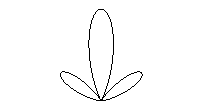
\includegraphics[width=\linewidth]{imgs/diag.pdf}
            \caption{}
            \label{fig:1:a}
        \end{subfigure}
        \begin{subfigure}[b]{.49\linewidth}
            \centering
            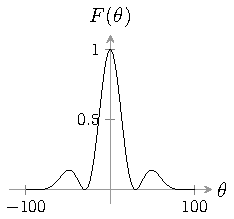
\includegraphics[width=\linewidth]{imgs/diag2.pdf}
            \caption{}
            \label{fig:1:b}
        \end{subfigure}
        \caption{Диаграмма направленности}
        \label{fig:1}
    \end{figure}
\end{center}


\textit{Коэффициент усиления} G определяется как произведение КНД на коэффициент полезного действия (КПД) антенны $\eta$
(или, точнее, всего антенного тракта):

\begin{equation}
    G = D\eta
    \label{eq:3}    
\end{equation}

Этот последний коэффициент в свою очередь есть отношение полной мощности $P_{\text{изл}}$, излучаемой антенной, к полной
мощности $P_{\text{подв}}$, подводимой к антенне, т.е.
\begin{equation}
    \eta =\frac{P_{\text{изл}}}{P_{\text{подв}}} = \frac{\int_{0}^{2 \pi} d \varphi \int_{0}^{\pi} P(\theta, \varphi) \sin \theta d \theta}{P_{\text{подв}}}
    \label{eq:4}    
\end{equation}

В силу принципа взаимности ДН и КНД антенны при ее работе в режиме передачи и в режиме приема совпадают.

Для адекватного описания \textit{приемной антенны} вводятся некоторые дополнительные характеристики. 
Одна из основных таких характеристик — эффективная площадь приема антенны $A$.

\textit{Эффективная площадь} приема $A$ определяется как отношение полной принимаемой антенной мощности 
$P_{\text{пр}}$ к плотности потока падающего
излучения $S_n$ в месте расположения антенны:
\begin{equation}
    A = \frac{P_{np}}{S_n}
    \label{eq:5}
\end{equation}
Величины $A$ и $D$ связаны соотношением
\begin{equation}
    A = \frac{\lambda^2}{4\pi}D.
    \label{eq:6}
\end{equation}

Цель настоящей работы заключается в экспериментальном определении КНД пирамидальной рупорной антенны с помощью так 
называемого зеркального метода (метода Парселла) и сравнении измеренного значения с рассчитанным теоретически. 
Зеркальный метод опирается на использование идеально (зеркально) отражающей плоской поверхности, расположенной в зоне 
Фраунгофера и ориентированной параллельно излучающей апертуре.

Согласно методу изображений отыскание отраженного поля, поступающего в антенну, сводится к нахождению поля, 
принимаемого от аналогичной зеркальной относительно отражающей плоскости излучающей антенны. В результате 
последовательного пересчета имеем: мощность, излучаемая гипотетической зеркальной антенной в единицу телесного угла 
в направлении на реальную антенну, равна $P_n = D P_{\text{изл}}/4\pi$, откуда плотность потока энергии в месте приема 
$S_n = P_n/4X^2 = D P_{\text{изл}}/(16\pi X^2)$, где $X$ — расстояние между антенной и отражающей плоскостью; наконец, 
мощность, принимаемая антенной, равна $P_{np} =A S_n =A D P_{\text{изл}}/(16\pi X^2)$. С учетом \ref{eq:6} окончательно 
получаем
\begin{equation}
    \frac{P_{np}}{P_{\text{изл}}} = \frac{D^2\lambda^2}{64\pi^2X^2}
    \label{eq:7}
\end{equation}

отсюда интересующая нас величина $D$ представляется в виде 
\begin{equation}
    D = \frac{8\pi X}{\lambda}\sqrt{\frac{P_{np}}{P_{\text{изл}}}}
    \label{eq:8}
\end{equation}

Таким образом, экспериментальное определение КНД требует нахождения отношения принимаемой зеркально отраженной мощности 
к мощности, излучаемой пирамидальной рупорной антенной. 

\begin{figure}[H]
    \centering
    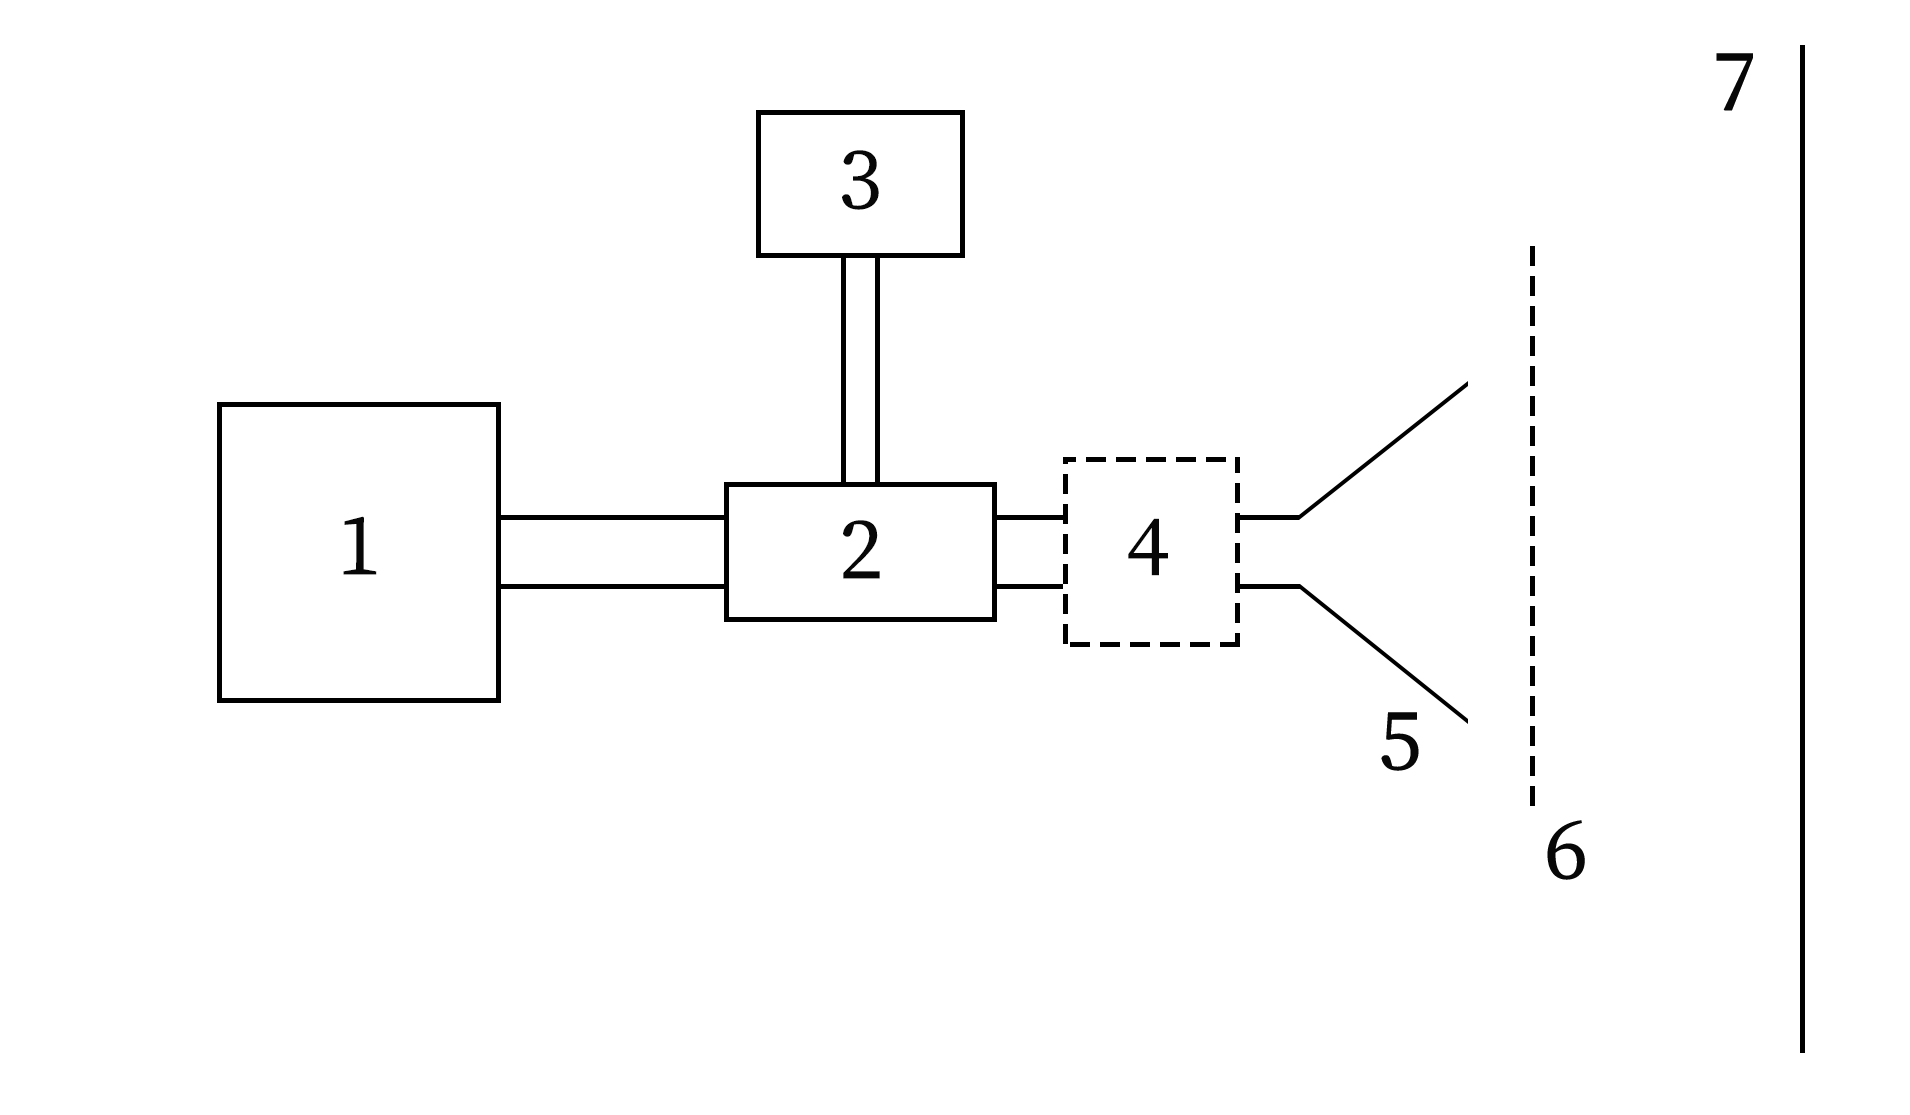
\includegraphics[width = 0.7\linewidth]{imgs/block.png}
    \caption{Блок-схема установки:  Схема установки: 1 – генератор, 2 – измерительная линия, 3 – амперметр, 4 –
    согласующее устройство, 5 – рупорная антенна, 6 - поглощающий щит, 7 – отражающий щит}
    \label{fig:2}
\end{figure}


Измерительная установка включает генератор СВЧ диапазона (длина излучаемой волны $\lambda \approx $ 3 см) с отдельным 
блоком питания, волноводный тракт с измерительной линией и амперметром к ней, пирамидальный рупор, отражающий щит, 
щит с поглощающим покрытием. Блок-схема установки на рис. \ref{fig:2}. 
Установка позволяет контролируемо менять расстояние $X + \Delta X$ между антенной и отражательным щитом в пределах
$\Delta X \approx $  100 см. 

Работа будет производиться в несогласованном режиме, когда специальной процедуры согласования не проводится. 
Учитывая отражения от конца подводящего тракта поле на оси волновода, отнормированное на 
амплитуду падающей волны, для некоторого фиксированного положения рупора запишется в виде
\begin{equation}
    E = 1e^{-ihx}+\Gamma_\kappa e^{i\varphi_\kappa} e^{ihx}+ \Gamma e^{e\varphi} e^{ihx}
    \label{eq:11}
\end{equation}
Смещение антенны на величину $\Delta X$ приведет к появлению в последнем члене дополнительного множителя $ e^{ i k_0
2\Delta X } $ , связанного с дополнительным набегом фазы в свободном пространстве. Поскольку 
$ \Gamma_{\kappa} \text{ и } \Gamma$ достаточно малы, то квадратичными величинами в первом приближении можно 
пренебречь. В результате для $ |E|^2 $ будем иметь 
\begin{equation}
    |E|^{2} \approx 1+2 \Gamma_{\kappa} \cos \left(2 h x+\varphi_{\kappa}\right)+2 \Gamma \cos \left(2 h x+\varphi+k_{0} 2 \Delta X\right)    
    \label{eq:13}
\end{equation}

Из уравнения выше и экспериментальных данных можно найти коэффициент $\Gamma$, тогда мы сможем определить интересующаю
нас величину $D$:
\begin{equation}
    D = \frac{8 \pi X}{\lambda} \Gamma.
    \label{eq:14}
\end{equation}



\textbf{Теоретический расчет КНД:}

В работе использовался рупор с размером апертуры $l_1\times l_2 = 9.2 \times 13.7 ~ cm$, подсоединенный к волноводу размером
$ 2.9 \times 1.02~cm. $

Чтобы рассчитать КНД рупорной антенны в зоне Фраунгофера, будем пользоваться интегралом Кирхгофа-Гюйгенса. Значение
компоненты поля в точке $P$, выражая через интеграл Кирхгофа :
\begin{equation}
    \Psi(P) = \frac{1}{4 \pi} \oint_{S}( \Psi \frac{\partial G}{\partial n} - G \frac{\partial \Psi}{\partial n})dS 
    \label{eq:1:1}
\end{equation}
где $P$ - точка наблюдения, $S$ - замкнутая поверхность, содержащая точку $P$,$n$ - внутренняя нормаль к $S$, $G$ - функция Грина свободного
пространства $$ G = \frac{1}{r} e^{i k r}. $$ 
Поверхность S выбираем так, чтобы она проходила через апертуру аннтены, а в отстальном пространстве удаляется на
бесконечность.
Рассматривая малые отклонения от центральной оси (т.е. в положении максимума), интеграл приводится к виду
\begin{equation}
    \Psi(P) = \frac{\Psi_0 ~exp(i k z_0) }{z_0 \lambda i} \iint_{\Sigma}~exp(\frac{i k}{2 z_0}(x^2+y^2))dxdy
    \label{eq:1:2}
\end{equation}
где $\Sigma$ - площадь апертуры. Интегралы Френеля, появляющиеся при дальнейшем решении не считаются аналитически, при
этом численный расчет показал, что интеграл дает значение, приблизительно равное площади апертуры ( Итегралы Френеля в
первом приближении дают значение площади апертуры). Таким образом, компонента поля в точке наблюдения:
\begin{equation}
    \Psi(P) \simeq \frac{\Psi_0}{z_0 \lambda i} S  e^{i k z_0}  
    \label{eq:1:3}
\end{equation}

Зная компоненту поля в максимуме, можно выразить плотность потока энергии:
\begin{equation}
    S_{max} = \frac{c}{8 \pi} \frac{\Psi_0^2 S^2}{r^2 \lambda^2} 
    \label{eq:1:4}
\end{equation}

Для расчета КНД, также необходима плотность потока энергии во всех направлениях. Для эквивалентного источника имеем:
\begin{equation}
    S_{r} = \frac{c}{8 \pi} \frac{\Psi_0^2 S}{r^2 \lambda^2} \frac{1}{4 \pi }
    \label{eq:1:5}
\end{equation}
Подставляя это в выражение для КНД, получаем:
\begin{equation}
    D = \frac{S_{max}}{S_r} = \frac{S}{\lambda^2} 4\ pi \simeq 156
    \label{eq:1:6}
\end{equation}
Однако, как мы увидим дальше, выражение \eqref{eq:1:6} дает завышенный КНД, что связано с неоднородностью распределения
поля на апертуре рупора.

\newpage
\section{Экспериментальная часть}
% Схема установки:
% \begin{figure}[H]
%     \centering
%     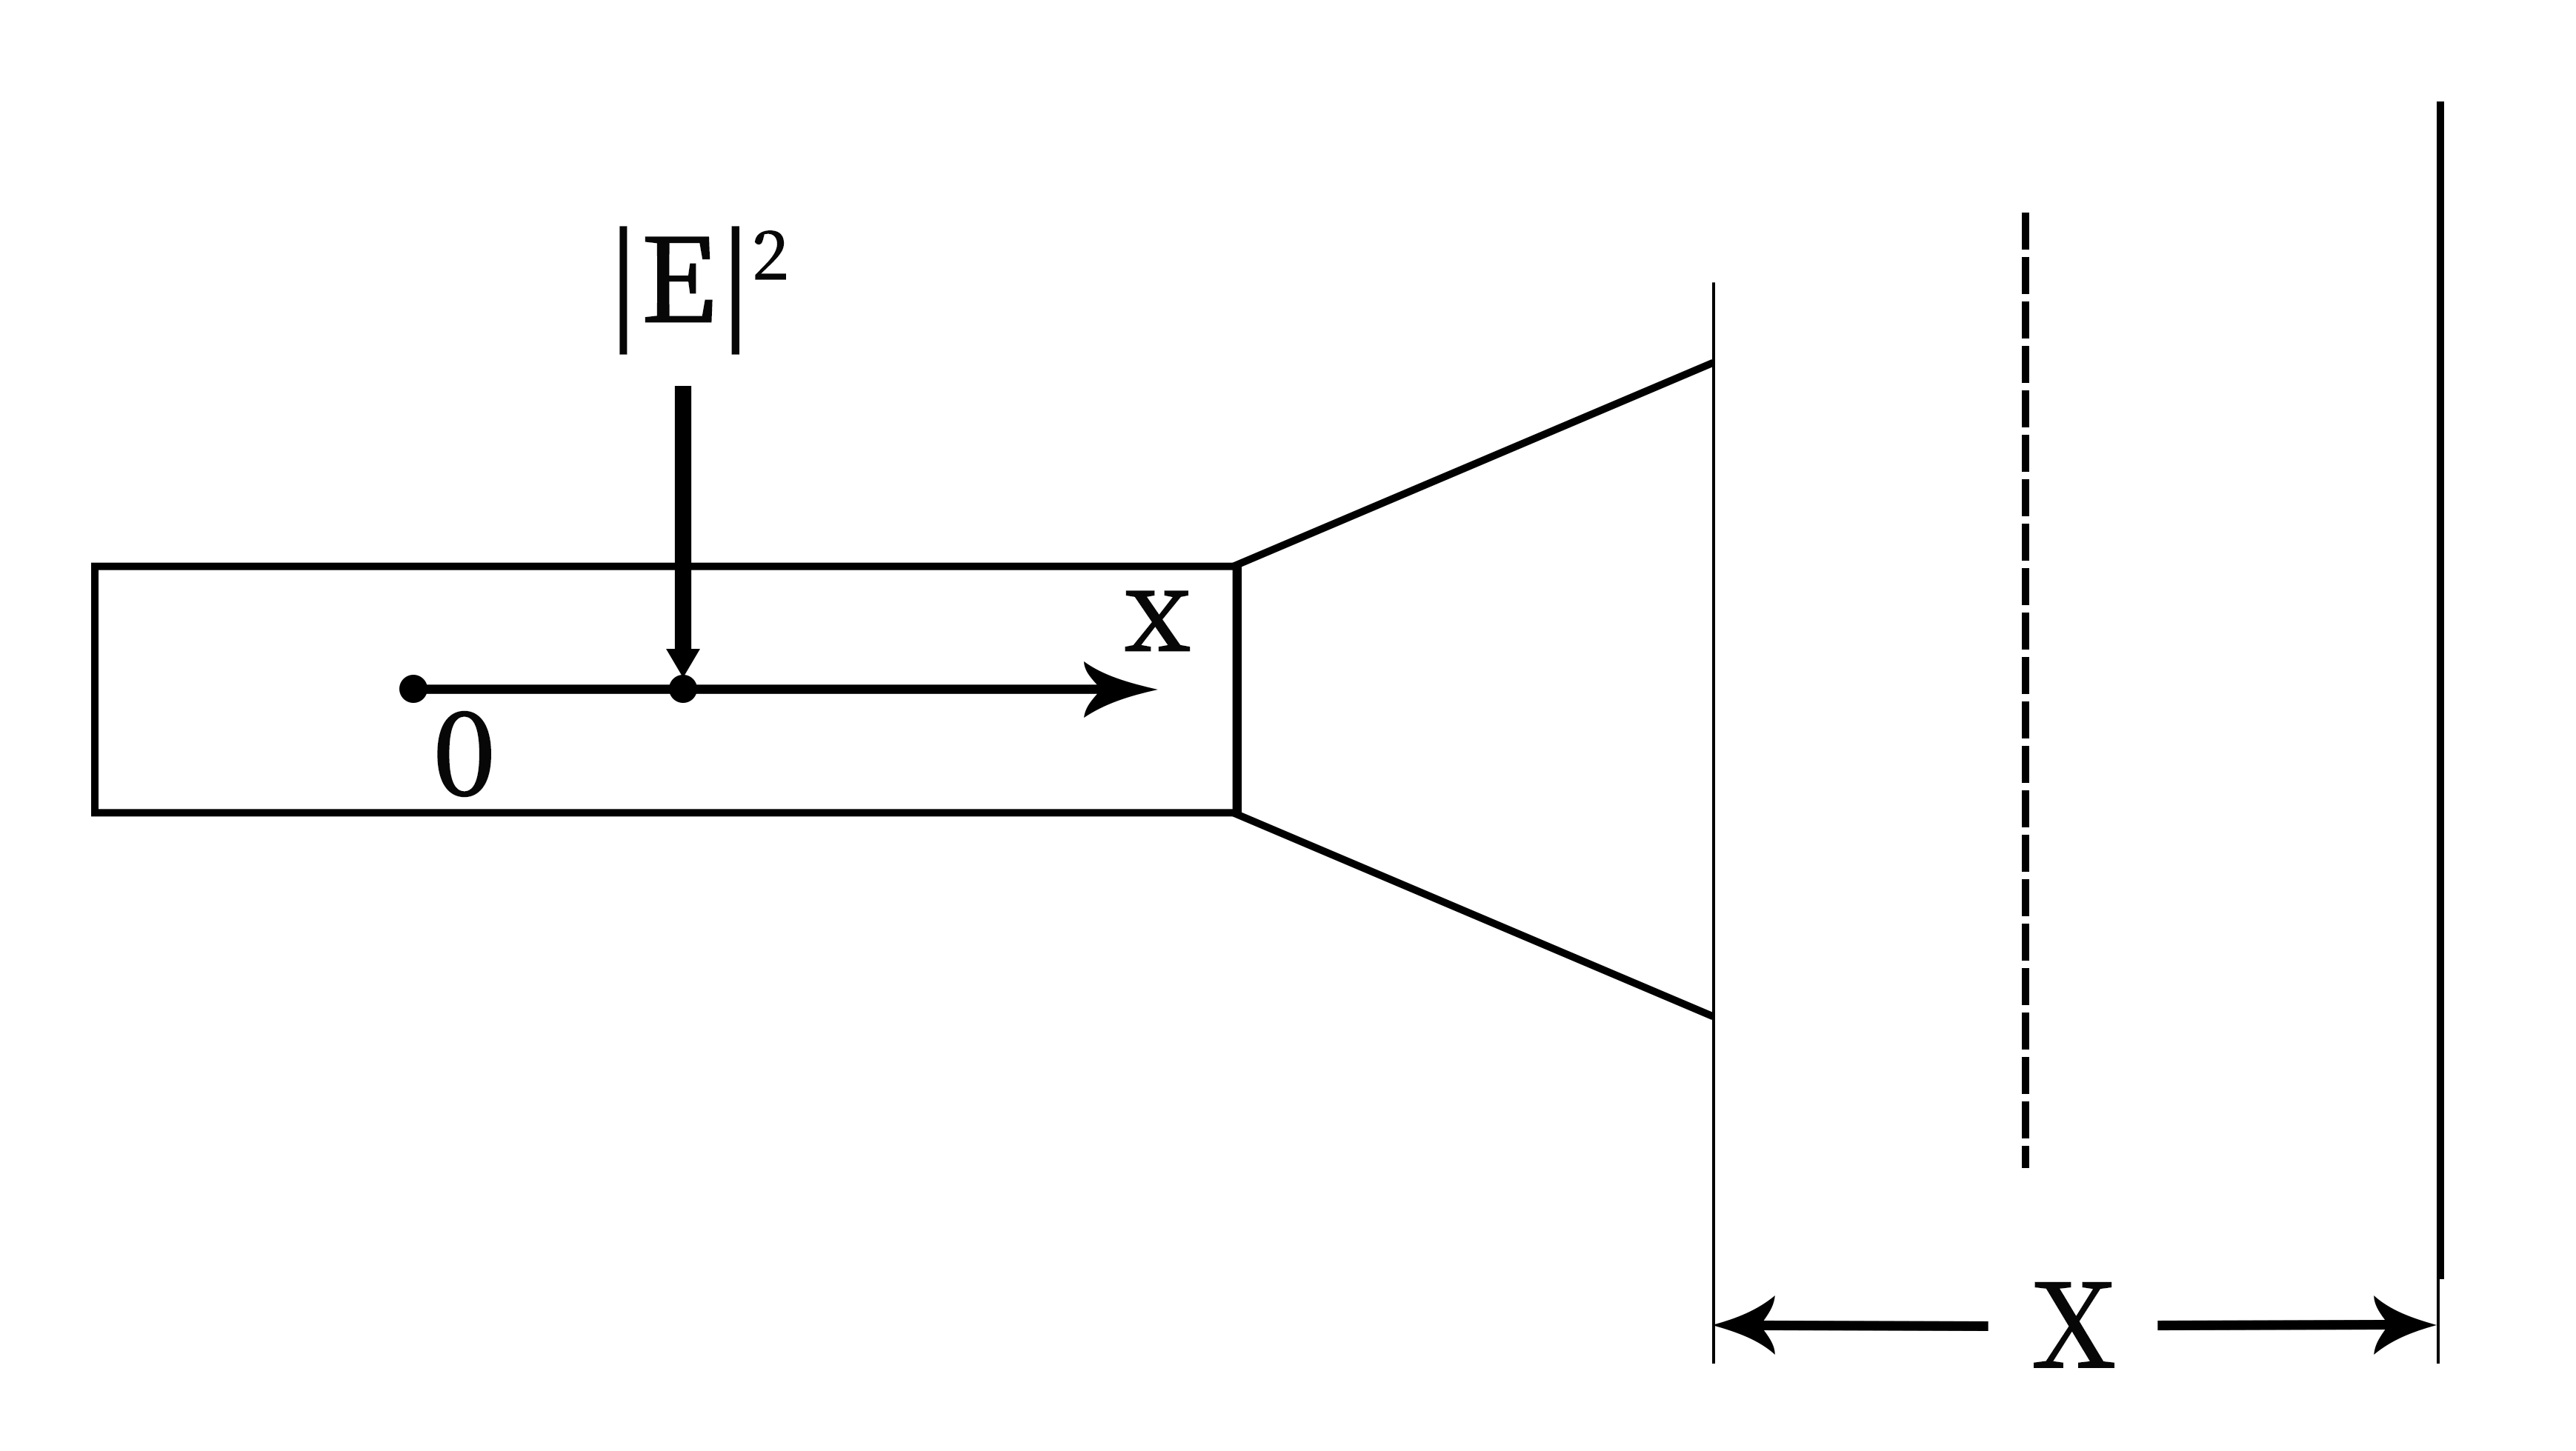
\includegraphics[width = 0.7\linewidth]{imgs/exp.png}
% \end{figure}
Оборудование: 
\begin{itemize}
    \item Генератор 
    \item Измерительные линейки 
    \item Амперметр квадратичного детектора 
    \item Рупорная антенна (апертура $l_1\times l_2 = 9.2 \times 13.7 ~ cm$)
    \item Поглощающий щит
    \item Отражающий щит
\end{itemize}
 
Начальное расстояние от отражающего щита до раскрыва рупора $X = 280~ cm$.

\textbf{Подготовка}

Для правильности проведения эксперимента, неоюходимо удостовериться, что экран находится в зоне Фраунгофера, т.е.:
\begin{equation}
    X = 280~cm~ >> \frac{max{l_1,l_2}}{\lambda} \simeq 63~cm 
    \label{eq:1:7}
\end{equation}

\subsection{Задание 1}
Перед антенной помещается щит с поглощающим покрытием, позволяя не учитывать отраженную от металлического щита часть
поля. Была снята зависимость интенсивности электрического поля $|E|^2$ от координаты внтури волновода $x$. Полученная
зависимость приведена на рис. \ref{fig:exp:1}.
\begin{figure}[h!]
    \centering
    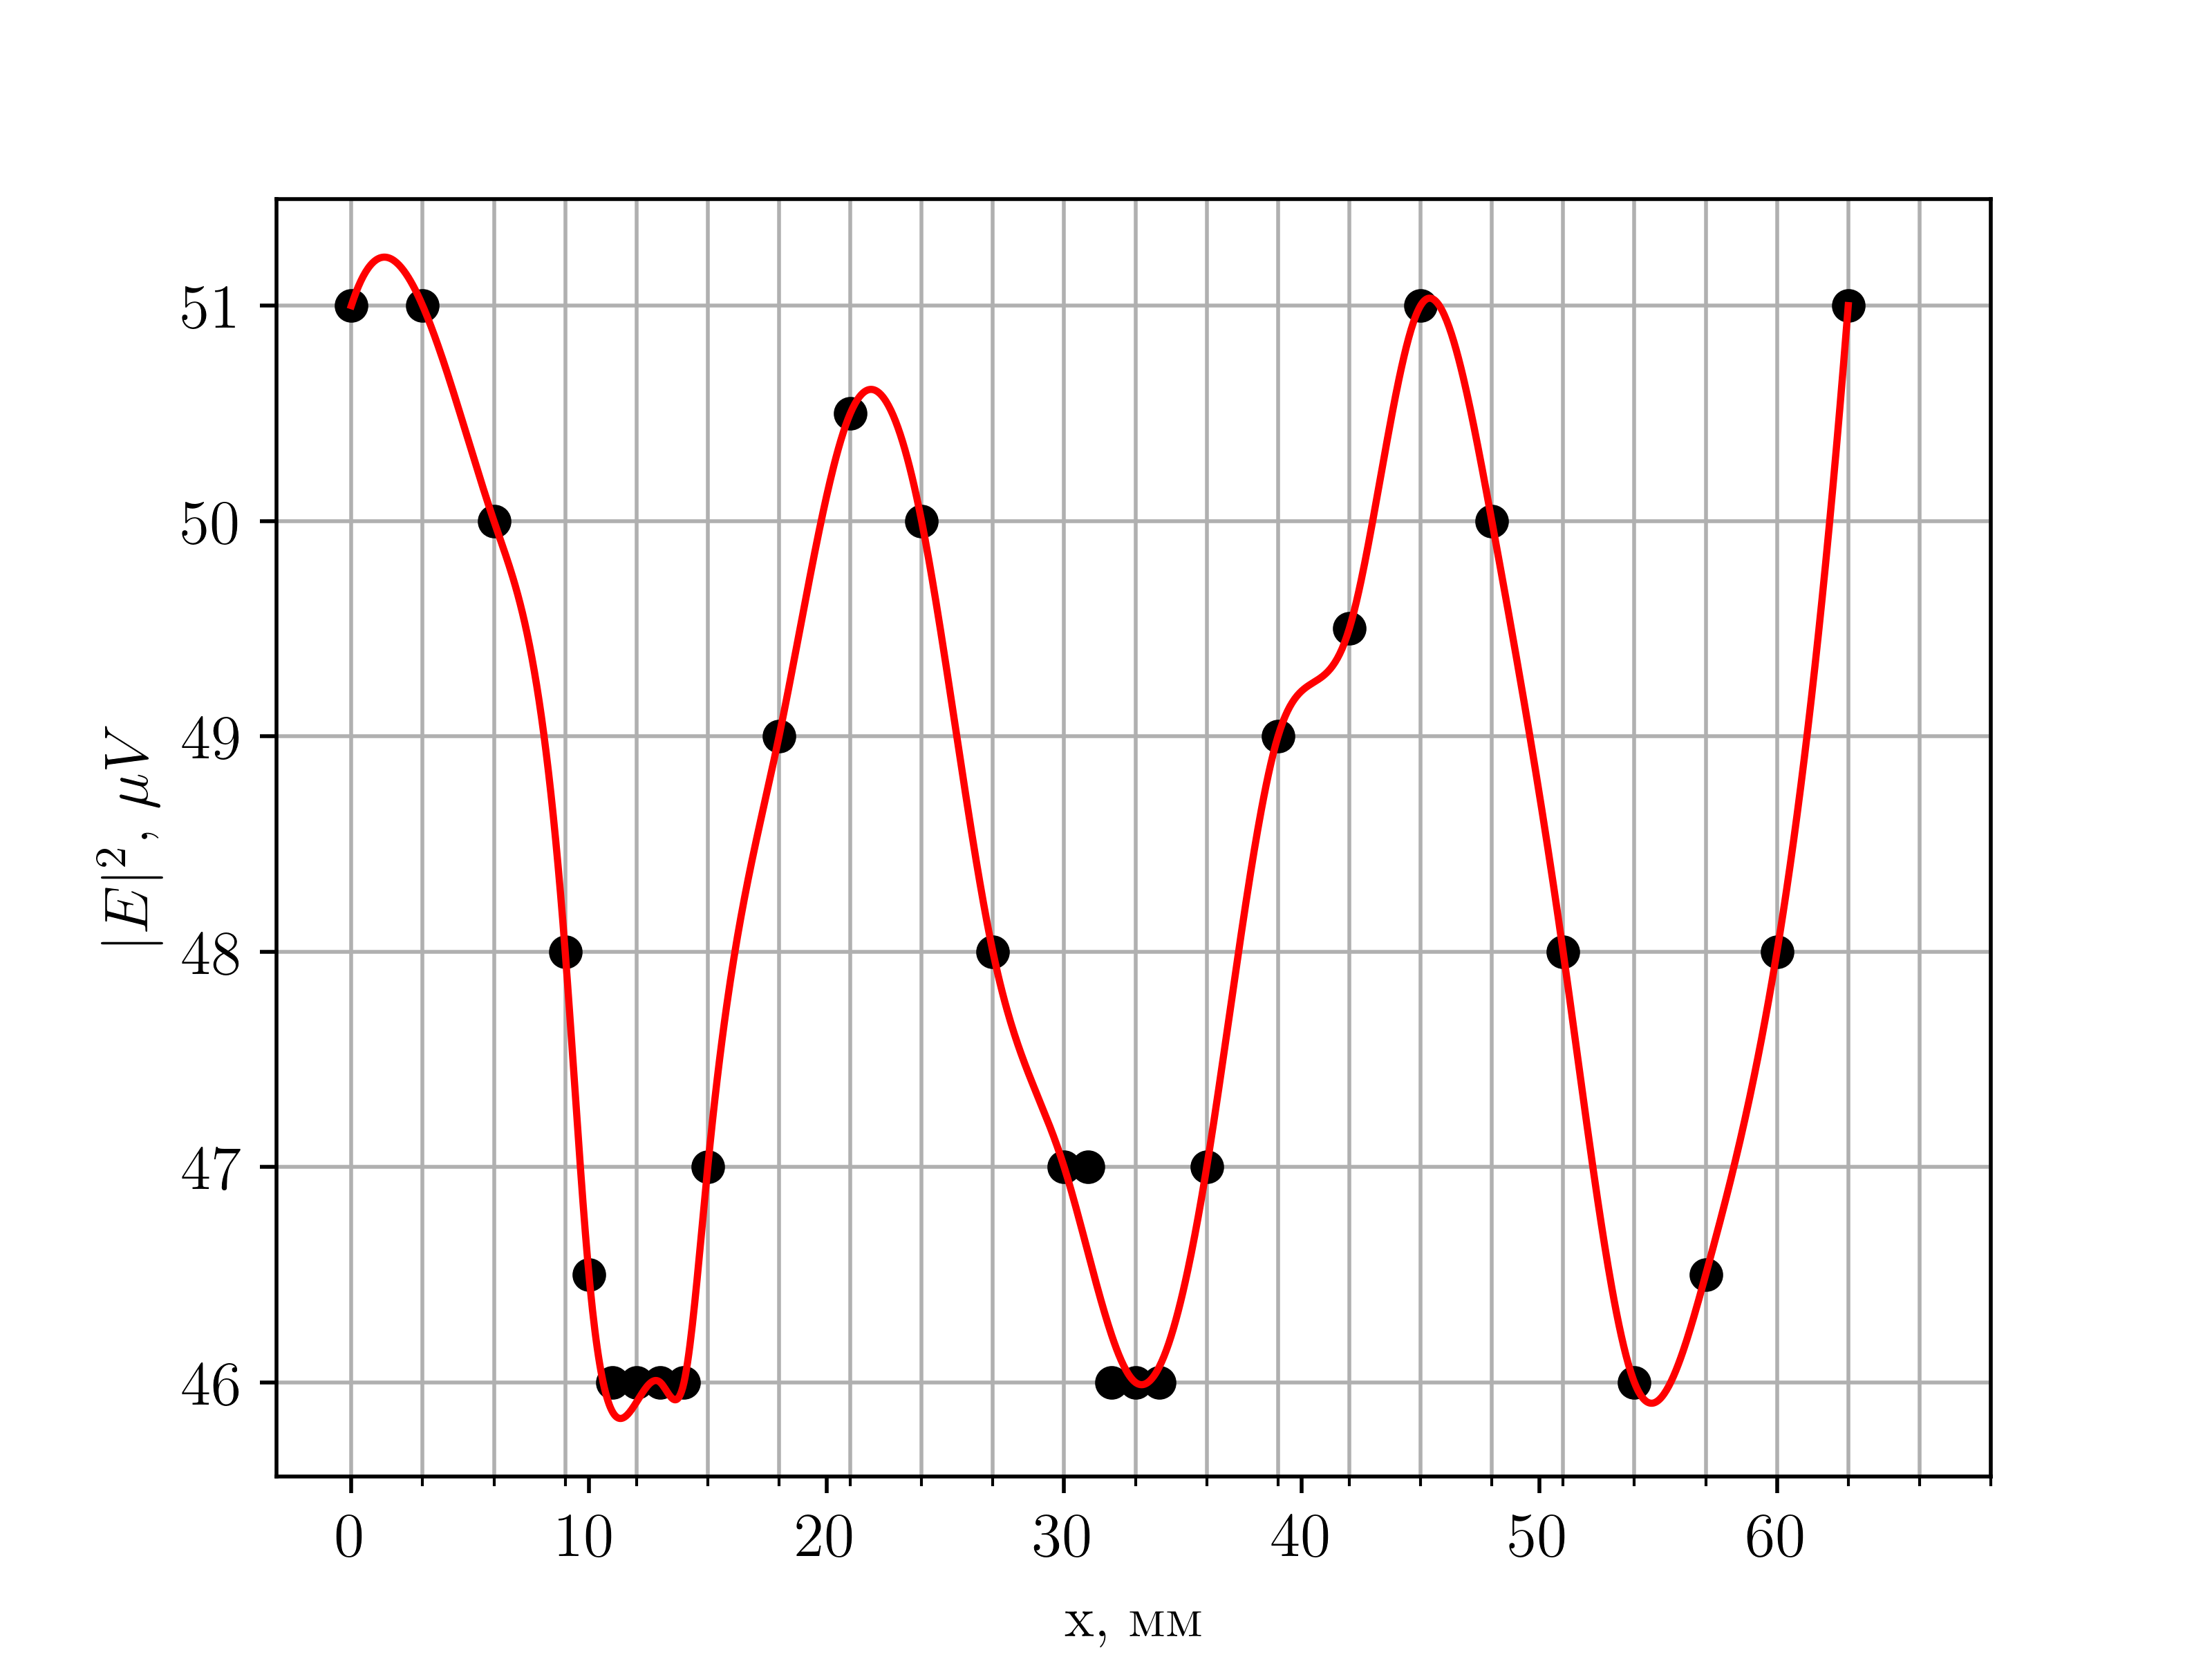
\includegraphics[width = 0.9\linewidth]{graphs/data111.png}
    \caption{Зависимость интенсивности $|E|^2$ от координаты x}
    \label{fig:exp:1}
\end{figure}

При отсутствии отраженной компоненты, уравнение \eqref{eq:13} упрощается к виду 
\begin{equation}
    |E|^2 \approx 1 + 2 \Gamma_{\kappa} \cos (2 h x + \varphi_{\kappa})
    \label{eq:15}
\end{equation}
Отсюда, по полученной зависимости $|E|^2(x)$ можно определить коэффициент $\Gamma_{\kappa}$:
\begin{equation}
    \Gamma_{\kappa} = \frac{|E_{max}|^2-|E_{min}|^2}{2( |E_{max}|^2+|E_{min}|^2 )} \approx 0.026
    \label{eq:16}
\end{equation}
Длина волны в волноводе $\lambda_{\text{в}}$ составила:
\begin{equation}
    \lambda_{\text{в}} \simeq 4.5 ~ cm    
\end{equation}
Зная $\lambda_{\text{в}}$, можно найти $\lambda$ в свободном пространстве:
\begin{equation}
    h^2 + \varkappa^2 = k^2  \Rightarrow \lambda = \frac{\lambda_{\text{в}}^2 4 a^2}{4a^2+\lambda_{\text{в}}^2} \simeq 3.21 ~cm    
\end{equation}
где $a = 2.29~cm$ - ширина волновода.
\subsection{Задание 2}
Найдя такое положение, что $\cos (2 h x +\varphi_{\kappa} )=0$ и зафиксировав его $(x = 2.6~cm)$, был убран отражающий щит и снималась
зависимость $|E|^2(\Delta X)$, где $\Delta X$ - смещение относительно металлического экрана. Полученная зависимоть
приведена на рис. \ref{fig:exp:2}.
\begin{figure}[h!]
    \centering
    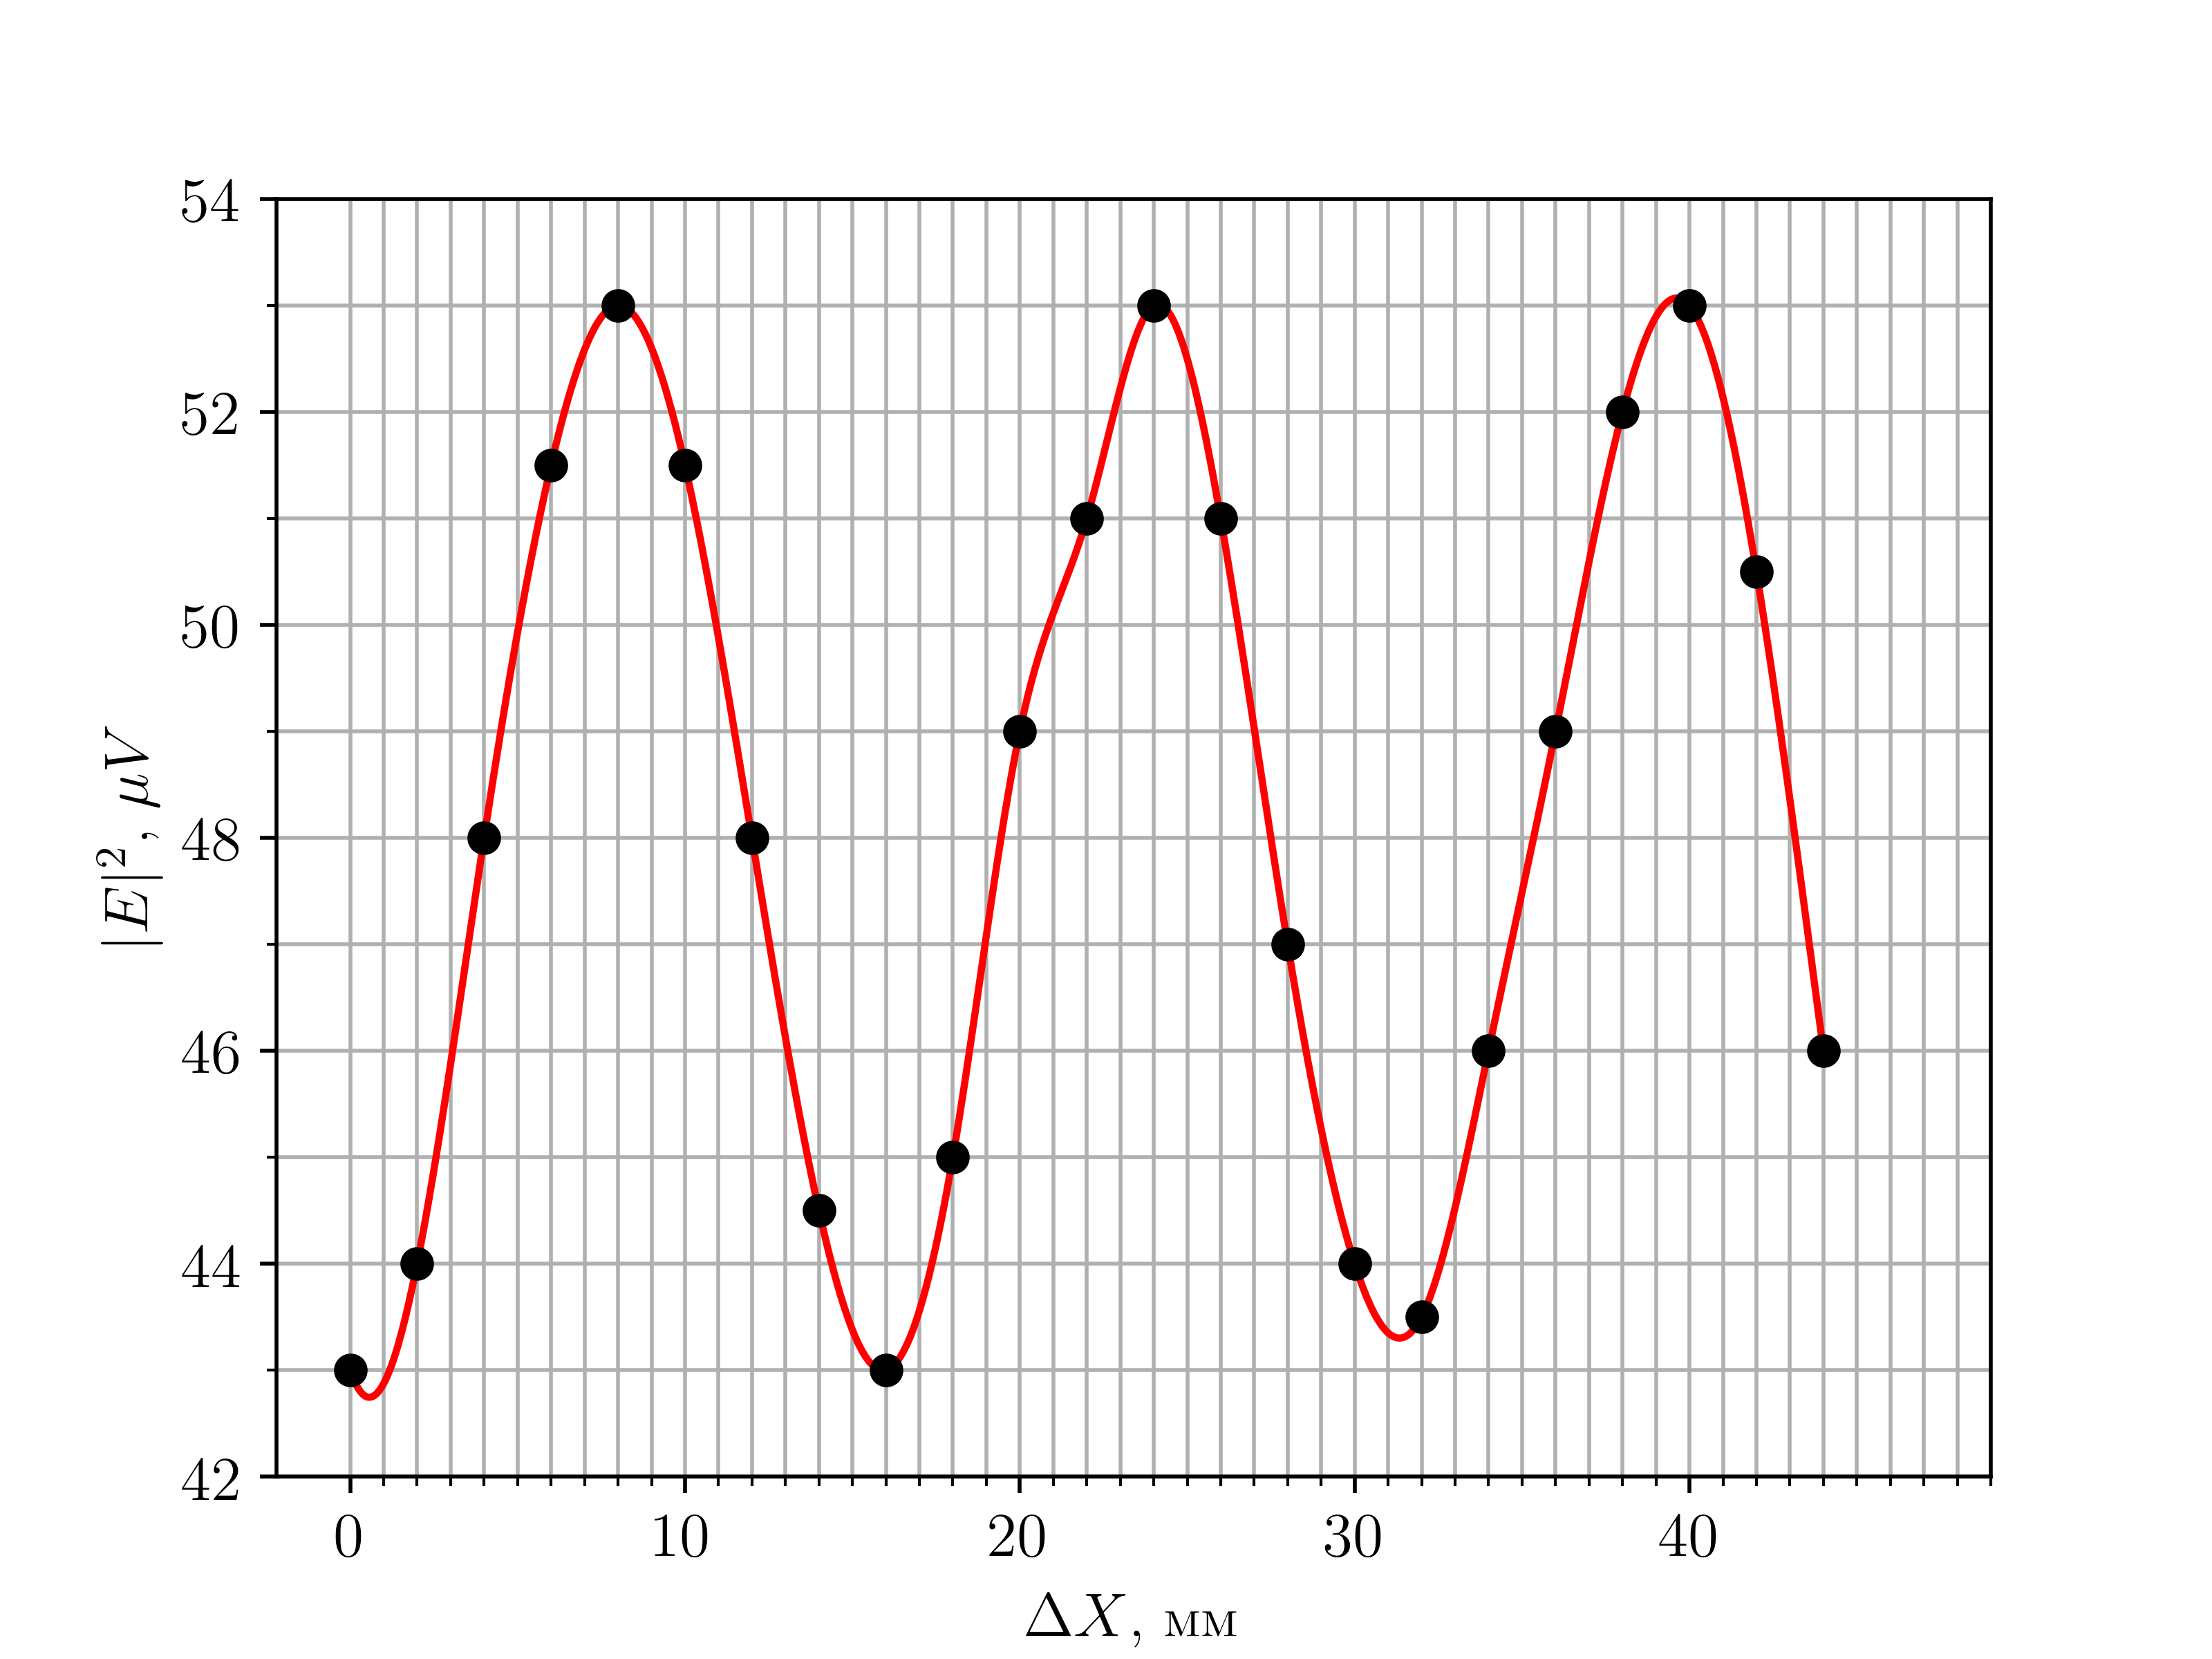
\includegraphics[width = 0.9\linewidth]{graphs/data222.png}
    \caption{Зависимость интенсивности $|E|^2$ от координаты смещения $\Delta X$}
    \label{fig:exp:2}
\end{figure}

Коэффициента отражения $\Gamma$ вычисляется аналогично первому заданию
\begin{equation}
    \Gamma = \frac{|E_{max}|^2-|E_{min}|^2}{2( |E_{max}|^2+|E_{min}|^2 )} \approx 0.05
\end{equation}
Тогда КНД, исходя и формулы \eqref{eq:14}
\begin{equation}
    D = \Gamma \frac{8 \pi X}{\lambda} \simeq 109.6    
\end{equation}


\subsection{Задание 3}
Меняя положение $X +\Delta X$ относительно отражающего щита, были измерены $|E_{max}|^2$ и $|E_{min}|^2$ и вычислен
КБВ в волноводе $\kappa = E_{min} / E_{max}$. Также был рассчитан коэффициент $\tilde{\Gamma} $:
\begin{equation}
    \tilde{\Gamma}(\Delta X)= \frac{1-\kappa (\Delta X)}{1+\kappa (\Delta X)} = \frac{1-\sqrt{K(\Delta X)}}{1+\sqrt{K(\Delta X)}} 
\end{equation}
Полученная зависимость приведена на рис. \ref{fig:exp:3}.
\begin{figure}[h!]
    \centering
    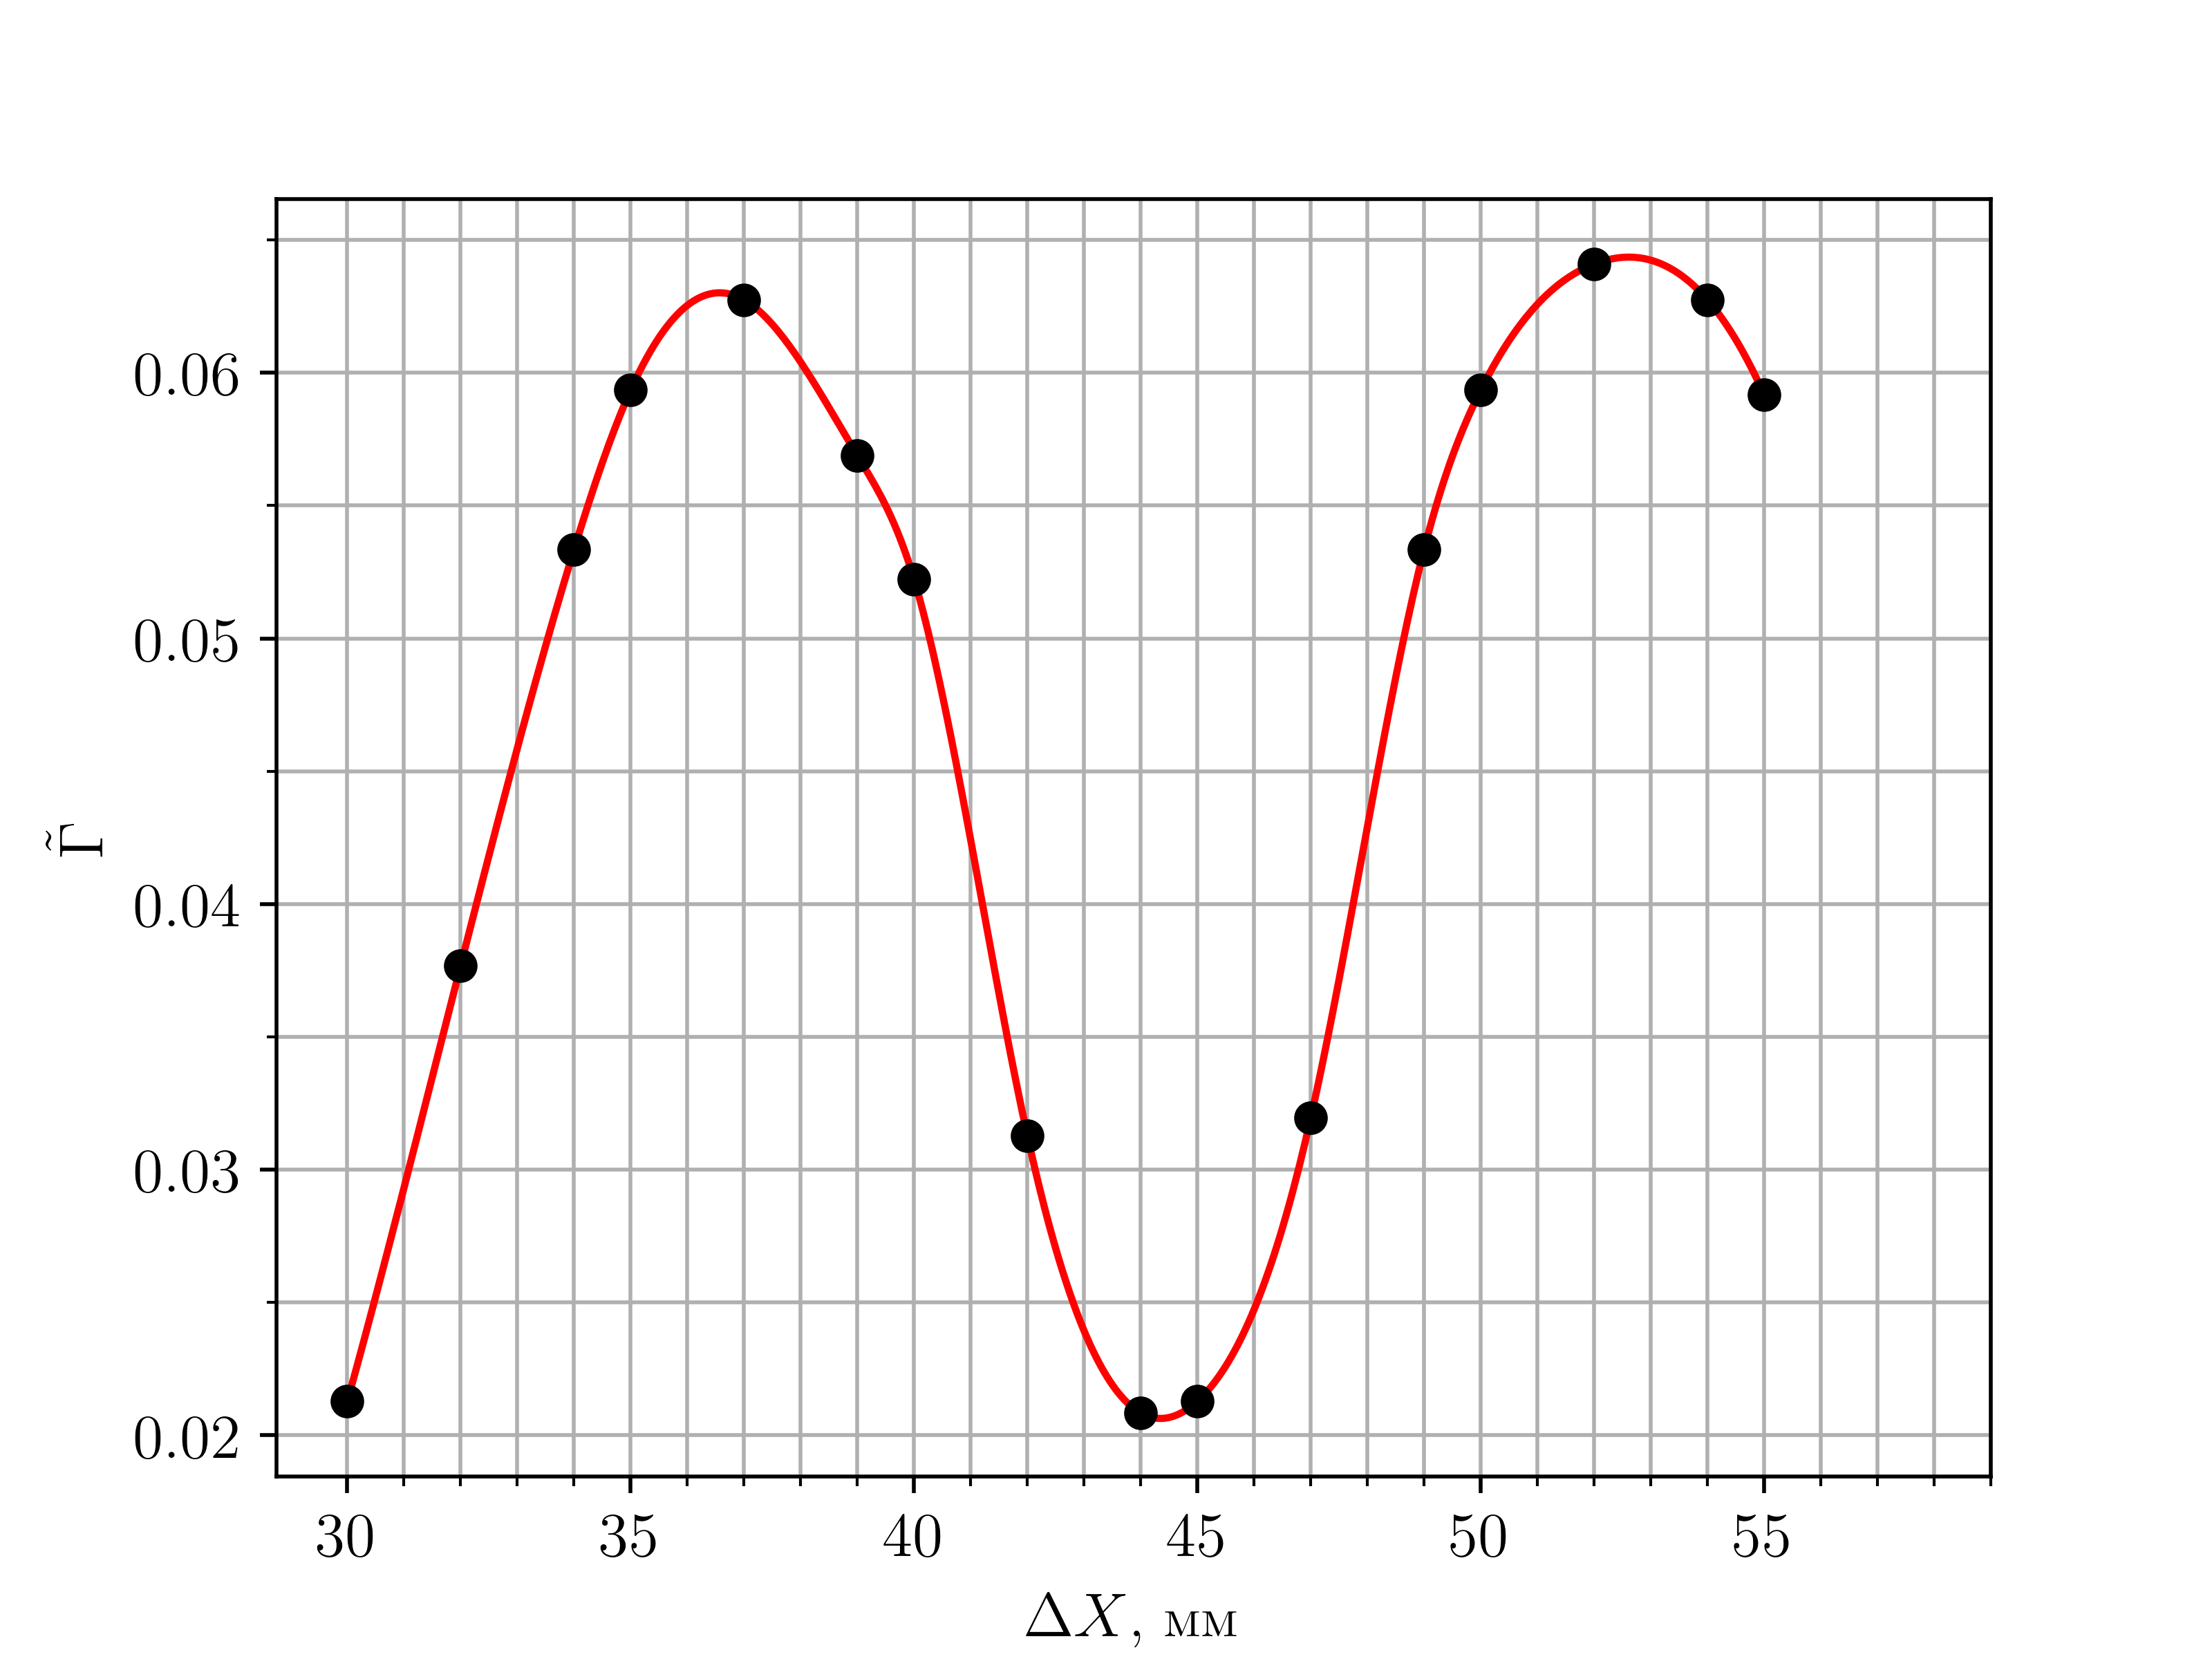
\includegraphics[width = 0.9\linewidth]{graphs/data33.png}
    \caption{Зависимость $\tilde{\Gamma}(\Delta X)$ }
    \label{fig:exp:3}
\end{figure}

Из полученного значения $\tilde{\Gamma}_{max} \simeq 0.064$ можно получить значение $\Gamma \simeq \tilde{\Gamma}_{max} -
\Gamma_{\kappa} \simeq 0.04$, откуда значение $D$: $$D \simeq 87.69$$ 

\textbf{Проверка предположения малости}

Ранее мы пренебрегли значениями $ \Gamma_{\kappa}^2,~ \Gamma^2,~ \Gamma_{\kappa} \Gamma $. Теперь, зная их, мы
можем убедиться в их малости: 
$$ \Gamma_{\kappa}^2 \simeq 0.026^2 \simeq 6.76 \cdot 10^{-4} $$
$$\Gamma^2 \simeq 0.05^2 \simeq 2.5 \cdot 10^{-3} $$
$$\Gamma_{\kappa} \Gamma \simeq 0.026 \cdot 0.05 \simeq 1.3 \cdot 10^{-3}$$


\subsection{Вывод}
В результате двух экспериментов были получены значения $D_1 = 109.6,~ D_2 = 87.7$, а также рассчитано теоретическое
значение $D_t = 156$. Расхождение экспериментальных значений связано с погрешностью измерений величин $E_{min}$ и
$E_{max}$. Расхождение же с теоретическим расчетом, связано с неоднородностью поля на апертуре рупора.
 
\end{document}